\subsubsection{2nd. Heliocentric stage }
In this section the equations and assumptions done in order to obtain the orbital elements of the trajectory will be explained. The objective of the calculations done regarding this stage is to find:
\begin{itemize}
\item $\Omega$ : Right ascension of the ascending node.
\item \textit{e}: Eccentricity.
\item \textit{i}: Inclination to the ecliptic plane.
\item \textit{a}: Semimajor axis.
\item $\omega$ : Argument of the perihelion. 
\end{itemize} 
As said previously, the times of departure and arrival are provided, together with the position of the planets. The steps to be followed to achieve the aim of this section are now explained.
\paragraph{Longitude, latitude and distance}
The position vector is defined as: 
\begin{equation}
\overrightarrow{r}=\left( x_k, y_k, z_k \right)
\end{equation}
Where: 
\begin{equation}
x_k = r cos\beta cos\lambda
\end{equation}
\begin{equation}
y_k=r cos\beta sin\lambda
\end{equation}
\begin{equation}
z_k=r sin\beta
\end{equation}
Then longitude, latitude and distance are computed with: 
\begin{equation}
r=|\overrightarrow{r}|
\end{equation}
\begin{equation}
\beta = \arcsin\left(\frac{z_k}{r}\right)
\end{equation}
\begin{equation}
\lambda = \arctan\left(\frac{y_k}{x_k}\right)
\end{equation}
The difference between $\lambda$ at the beginning and at the end of the trajectory is an important magnitude that will be used. Taking into account that subscript 1 refers to the start position and subscript 2 to the end: 
\begin{equation}
\Delta \lambda = \lambda _2 - \lambda _1
\end{equation}
\paragraph{Inclination, right ascension of the ascending node and true anomaly variation}
Trigonometry has to be used to compute this elements. A general case will be considered, that is to say, that no assumption will be done on whether the two planets are on the ecliptic or not. As shown in reference \cite{PCA}, the equations to be used are: 
\begin{equation}
\cos \Delta\theta = \sin\beta _1 \sin\beta _2 + \cos\beta _1 \cos\beta _2 \cos\Delta\lambda
\end{equation} 
\begin{equation}
\sin A=\cos\beta _2 \frac{\sin\Delta\lambda}{\sin\Delta\theta}
\end{equation}
\begin{equation}
\cos i=\sin A\cos\beta_1
\end{equation}
\begin{equation}
\sin l=\frac{\tan\beta _1}{\tan i}
\end{equation}
\begin{equation}
\tan \sigma = \frac{\tan \beta _1}{\cos A}
\end{equation}
\begin{equation}
\Omega = \lambda _1-l
\end{equation}
\paragraph{Eccentricity, semimajor axis and true anomaly of the starting point}
With the aim of obtaining this data three equations can be stated. Due to the complexity of the equations, the resolution will be done iteratively. Two cases will be considered: elliptic and hyperbolic. Its equations and iteration process are now shown: 
\begin{itemize}
\item Elliptic trajectory:
The equations of the elliptic trajectory are: 
\begin{equation}
e=\frac{r_2-r_1}{r_1\cos\theta _1-r_2\cos(\theta_1+\Delta\theta)}
\end{equation}
\begin{equation}
a=\frac{r_1\left(1+e\cos\theta _1\right)}{1-e^2}
\end{equation}
\begin{multline}
t_2-t_1=\frac{365.25}{2\pi}a^\frac{3}{2}\Bigg(2\arctan\bigg(\sqrt{\frac{1-e}{1+e}}\tan\frac{\theta _1 +\Delta\theta}{2}\bigg)\\-\frac{e\sqrt{1-e^2}\sin (\theta _1+\Delta\theta)}{1+e\cos (\theta _1+\Delta\theta}-2\arctan\bigg(\sqrt{\frac{1-e}{1+e}}\tan \frac{\theta _1}{2}\bigg)+\frac{e\sqrt{1-e^2}\sin \theta _1}{1+e\cos \theta1}\Bigg)
\end{multline}

The iteration process done to solve the equations will deal with the difference between the time of the mission calculated and the real time of the mission, that is a known value. An error criteria $\epsilon$ is defined as the convergence value. The flow chart of this iteration is shown in Figure \ref{Floweliptic}.
\begin{figure}[H]
\centering
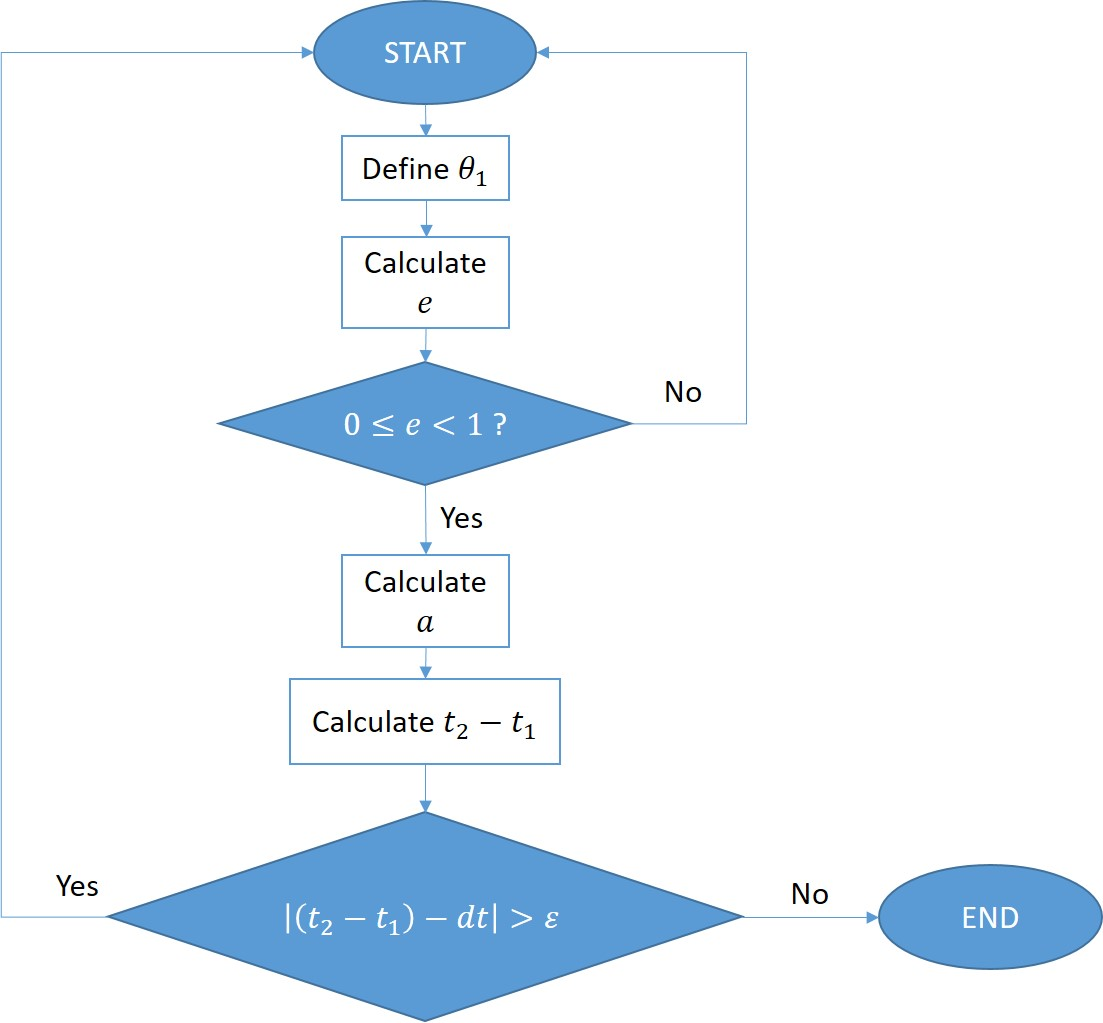
\includegraphics[width=0.8\textwidth]{././images/flowcharteliptic.jpg} 
\caption{Flow chart for the elliptic trajectory resolution.}
\label{Floweliptic}
\end{figure}
\item Hyperbolic trajectory: The equations of the hyperbolic trajectory are:
\begin{equation}
e=\frac{r_2-r_1}{r_1\cos\theta _1-r_2\cos(\theta_1+\Delta\theta)}
\end{equation}
\begin{equation}
a=\frac{r_1\left(1+e\cos\theta _1\right)}{e^2-1}
\end{equation}
\begin{multline}
t_2-t_1=\frac{365.25}{2\pi}a^\frac{3}{2}\Bigg( \frac{e\sqrt{e^2-1}\sin (\theta _1 +\Delta\theta)}{1+e\cos (\theta _1+\Delta\theta)} - \\
ln \left| \frac{\tan \frac{\theta _1 +\Delta\theta}{2}+\sqrt{\frac{e+1}{e-1}}}{\tan \frac{\theta _1 +\Delta\theta}{2} -\sqrt{\frac{e+1}{e-1}}} \right| -\frac{e\sqrt{e^2-1}\sin \theta _1}{1+e\cos \theta _1}+ln\left| \frac{\tan \frac{\theta _1}{2}+\sqrt{\frac{e+1}{e-1}}}{\tan \frac{\theta _1}{2}-\sqrt{\frac{e+1}{e-1}}}\right| \Bigg)
\end{multline}
The resolution is similar to that of the elliptic case, but the acceptable values of the eccentricity change. The flow chart is shown in Figure \ref{Flowhyp}.
\begin{figure}[H]
\centering
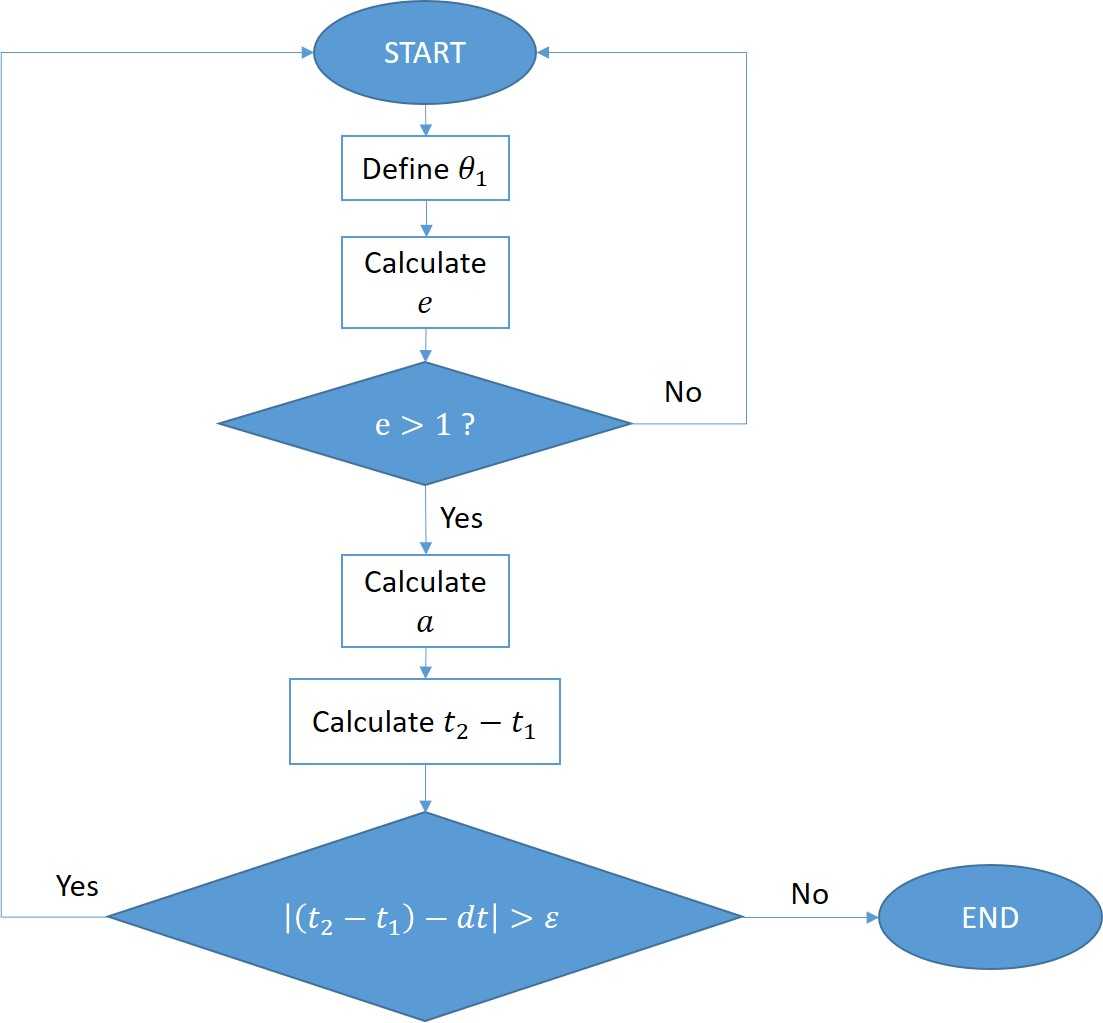
\includegraphics[width=0.8\textwidth]{././images/flowcharthyp.jpg} 
\caption{Flow chart for the hyperbolic trajectory resolution.}
\label{Flowhyp}
\end{figure}
\end{itemize}
\paragraph{Argument of the perihelion} 
The only remaining orbit element that needs to be computed is $\omega$. It can be calculated using results from the previous steps:
\begin{equation}
\omega = 2\pi - (\theta _1 - \sigma )
\end{equation}

\paragraph{Spacecraft velocity}
Sphere Of Influence (SOI), departure and arrival velocities are computed under the following theoretical background.

First of all, a geocentric coordinates system is considered, the orbital plane \textit{$PQW(\bar{x})$}





